\documentclass[12,a4paper]{article}
\usepackage{classiccomputing}

\newcommand\postertype{lightgray}

\begin{document}

\makecclogo

\author{LaF0rge} % owner of the device, also used as "Author" in PDF export
\title{7-E Communications Talking Head}
\def\subtitle{ISDN Bildreporter-Telefon}
\def\introduction{Markteinführung 1997}
\makeheader{33}{40} % title size 33, subtitle size 40

\includeimage {images/7e-talking_head.jpg}{0.35}

\makebullets{
    Land: Vereinigtes Königreich \newline
    Hersteller: 7-E Communications (Systemintegrator) \newline
    Codec-Einheit: Motion Media 8120-AC \newline
    Kaufpreis: ca. 70.000 DM \newline
    Verbreitung: über 400 Stück \newline

    Videotelefon für TV-Reporter im Außeneinsatz \newline

    Audioeingang: XLR (1x Mikrophon + 2x Line-In) \newline
    Videoeingang: BNC + Cinch (composite) \newline
}

\makemain{
ISDN-Bildtelefonie ermöglichte es Fernsehreportern erstmals ohne riesiges Gerät wie TV-Übertragungswagen relativ schnell Live in Bild und Ton zu berichten.  Alles was nötig war, ist ein ISDN-Telefonanschluss, oder alternativ auch ein Satellitentelefon (wie z.B. Inmarsat).  Dies ermöglichte Übertragung unter schwierigen Bedingungen, mit Equipment aus dem persönlichen Reisegepäck.
\newline
\newline
Mit dem 7-E Talking Head TH-1 und TH-2 wurden z.B. Berichte für CNN Übertragen, u.a. aus dem Irak-Krieg 2003.
\newline
\newline
Im Gegensatz zum ISDN-Bildtelefon auf dem Schreibtisch ist im 7-E Talking Head keine Kamera und kein
Mikrofon eingebaut.  Vielmehr wurde Bild+Ton von der vorhandenen Videokamera + Mikrofon des Reportage-Teams über entsprechende XLR- und BNC-Buchsen zugeführt.
}

%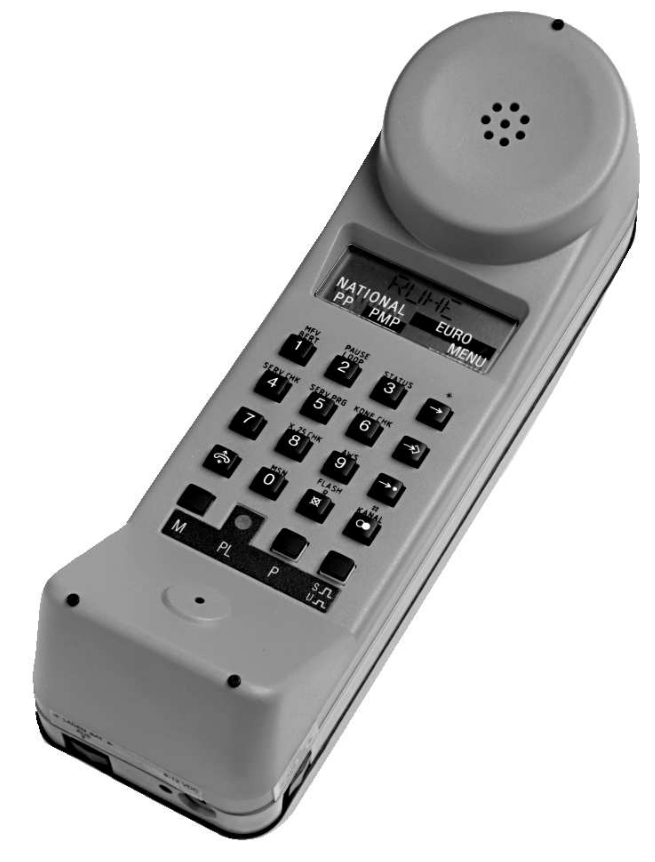
\includegraphics[width=0.5\linewidth]{images/prtel93i.png}

\makefooter

\end{document}
